\chapter{Measurement of the inclusive $t\bar{t}+\gamma$ cross-section}\label{chap-crosssection}

\section{Signal Definition and Background Processes}

\subsection{Signal definition}

\begin{figure} \label{fig-signalphotonplot}
\begin{center}
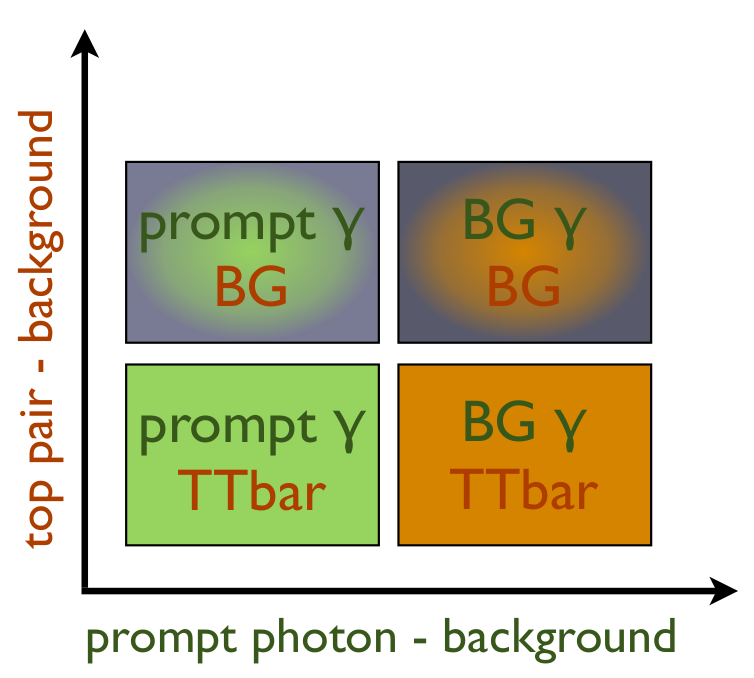
\includegraphics[scale=0.33]{Figures/SignalPhotonPlot.png}
\caption{Graphic representation of the signal and background definitions \cite{MishaSignalDefinition}.}
\end{center}
\end{figure}

\subsection{Background processes}

\begin{figure}
\begin{center}
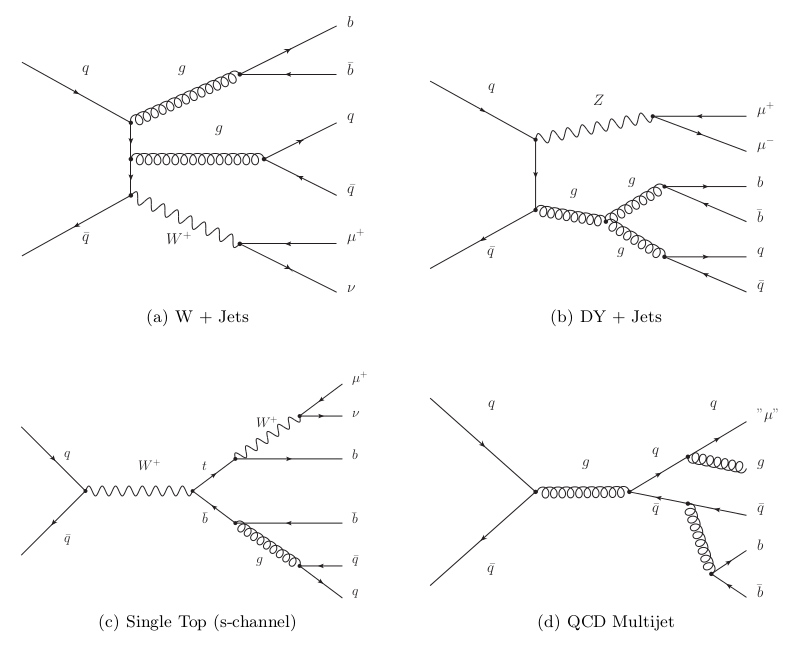
\includegraphics[width=\textwidth]{Figures/BackgroundDiagrams.png}
\caption{Examples of Feynman graphs of the considered $t\bar{t}$ backgrounds. QCD showering is necessary in all cases to obtain the required jet multiplicity \cite{ttgammabackgroundestimation}.}
\end{center}
\end{figure}

\begin{figure}\label{fig-AnalysisFlowChart}
\begin{center}
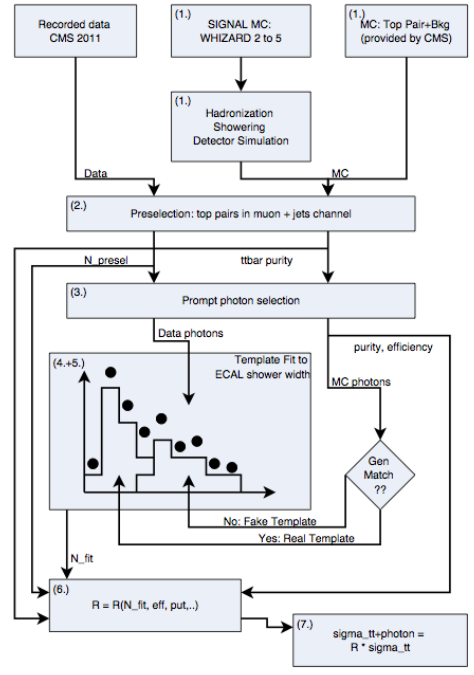
\includegraphics[width=0.75\textwidth]{Figures/AnalysisFlowChart.png}
\caption{Flow chart showing each stage of the analysis. The box numbers represent the outlined
analysis steps.}
\end{center}
\end{figure}

\subsection{Backgrounds of photon signature}

\begin{figure} \label{fig-BackgroundISR}
\begin{center}
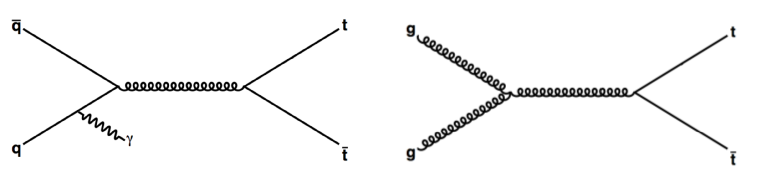
\includegraphics[width=\textwidth]{Figures/BackgroundISR.png}
\caption{Background of photon identification: Initial state radiation (ISR). Left: Quark fusion. Right: Gluon fusion does not give rise to ISR (based on \cite{photonbackgrounds}).}
\end{center}
\end{figure}


\begin{figure} \label{fig-BackgroundFSR}
\begin{center}
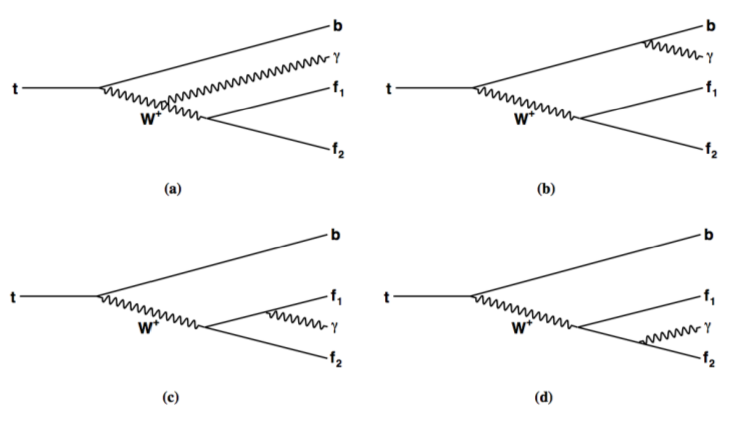
\includegraphics[width=\textwidth]{Figures/BackgroundFSR.png}
\caption{Background of photon identification: Final state radiation (FSR). All charged particles in the top-pair decay tree contribute to FSR \cite{photonbackgrounds}.}
\end{center}
\end{figure}

\section{$t\bar{t}+\gamma$ Signal Simulation}

WHIZARD

then

MADGRAPH

Factorised matrix element 

\section{Phase Space Overlap Removal} \label{sec-PhaseSpaceOverlapRemoval}

Events of the $t\bar{t}+\gamma$ process lie within a small region of $t\bar{t}$ phase space, and thus our signal sample events are expected to overlap with TTJets events in the case where a hard photon is radiated by initial state quarks, top quarks, b quarks, W and its decay products: electrons, muons, and their corresponding neutrino. In order to prevent the double counting of events we apply an overlap removal procedure to remove such events from our TTJets samples. In order for an event to be considered as overlapping with TTGamma, an event has to have at least one generator-level photon with the following properties:

\begin{itemize}
	\item p$_T(\gamma) > 13$ GeV
	\item $|\eta| < 3.0$
	\item Only gluons, bosons, or leptons are in the parents list. This ensures that photons from $\pi^0$ decays are not considered as signal
	\item $\Delta R(\gamma, other) > 0.2$ where other particles include leptons, b quarks and final state particles (hadrons, charged leptons, photons) with transverse momenta above $5 \GeV$.
\end{itemize}

The last cut is implemented in order to suppress photons from showers. In such cases the information from the parent particle will show that a photon is radiated by an electron, however the photon may be collinear with it. In particular in TTJets di-lepton events, such as described in this analysis, where a considerable fraction of the reconstructed photons comes from electrons radiating photons.

 Similarly, we also observe an overlap between Z+Jets and ZGamma processes, and between W+Jets and WGamma samples, for the same reasons as described above. The phase space overlap removal procedure is applied on Z+Jets and W+Jets samples to remove events containing generator-level photons. Events containing generated photons are removed in the case in which they are from initial state radiation (emitted from the colliding partons) or final state radiation (emitted from W or Z bosons or their decay products), since these are already included in the WGamma and ZGamma simulations. The overlap removal procedure removes approximately one percent of the events in the W+Jets sample, and approximately three to four percent of the events from the TTJets and Z+Jets samples.

\begin{figure} \label{fig-photonphasespace}
\begin{center}
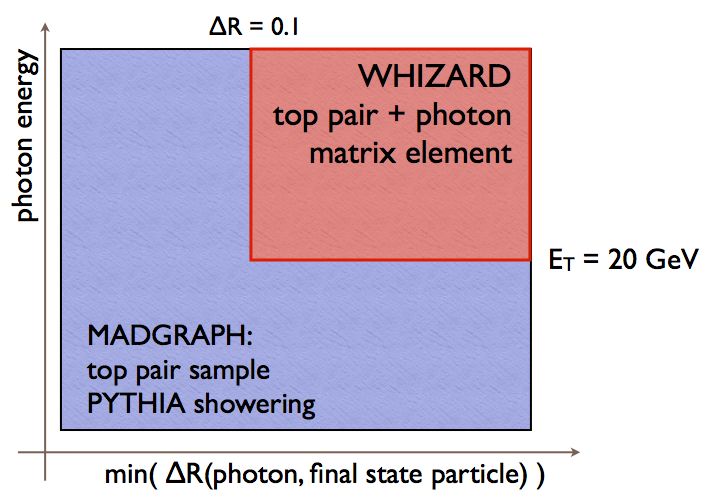
\includegraphics[scale=0.5]{Figures/photonphasespace.png}
\caption{}
\end{center}
\end{figure}

\section{Event Selection} \label{sec-EventSelection}

\section{Photon Purity Estimation} \label{sec-PhotonPurityEstimation}

\section{Signal Acceptance Calculation} \label{subsec-SignalAcceptanceCalculation}

Acceptance calculation for this analysis differs from usual inclusive cross section measurements because we measure ratio of cross sections. The event selection is chosen to make use of this fact: two steps (top selection and photon selection) are done sequentially. For the inclusive $t\bar{t}$ process, we start with number of generated events (within some fiducial phase space) and count how many events are left after top event selection. The acceptance times efficiency is defined for the $t\bar{t}$ top selection as:

\begin{equation}
	\epsilon^{t\bar{t}}_{top} \cdot A^{t\bar{t}}_{top} = \frac{N_{t\bar{t}.preselection}}{N_{t\bar{t}.generated}} 
\end{equation}

This gives the acceptance times efficiency of the inclusive $t\bar{t}$ process to be $\epsilon^{t\bar{t}}_{top} \cdot A^{t\bar{t}}_{top} =   \pm  (stat.)$ in the di-muon channel, $\epsilon^{t\bar{t}}_{top} \cdot A^{t\bar{t}}_{top} =  \pm  (stat.)$ in the di-electron channel, and $\epsilon^{t\bar{t}}_{top} \cdot A^{t\bar{t}}_{top} =  \pm  (stat.)$ in the mixed final state.

The same can be done for the $t\bar{t}+\gamma$ (signal sample). To get the acceptance times efficiency we have to divide the number of events passing top selection by the total number of events considered. However, in this case we have to choose what we take as the denominator. The signal $t\bar{t}+\gamma$ sample is inclusive, but theoretical calculations for the cross section are done for final states with 1 and 2 leptons \cite{QCDCorrectionsttgamma2011}. To make comparison with theory easier we consider the fiducial space for signal when 1 or 2 leptons are present. The $t\bar{t}+\gamma$ acceptance times efficiency of the top selection is defined for the signal samples with 1 or 2 leptons as:

\begin{equation}
	\epsilon^{t\bar{t}+\gamma}_{top} \cdot A^{t\bar{t}+\gamma}_{top} = \frac{N_{t\bar{t}+\gamma.preselection(1lor2l)}}{N_{t\bar{t}+\gamma.generated(1lor2l)}} 
\end{equation}

Giving the acceptance times efficiency of the inclusive $t\bar{t}+\gamma$ process to be $\epsilon^{t\bar{t}+\gamma}_{top} \cdot A^{t\bar{t}+\gamma}_{top} =   \pm  (stat.)$ in the di-muon channel, $\epsilon^{t\bar{t}+\gamma}_{top} \cdot A^{t\bar{t}+\gamma}_{top} =  \pm  (stat.)$ in the di-electron channel, and $\epsilon^{t\bar{t}+\gamma}_{top} \cdot A^{t\bar{t}+\gamma}_{top} =  \pm  (stat.)$ in the mixed final state.

The acceptance and efficiency for the $t\bar{t}+\gamma$ sample includes a term for photon selection. This is found based on the ratio of the number of events in $t\bar{t}+\gamma$ passing photon selection and the reconstructed photon matched to a generated photon over the number of events passing the top selection. The $t\bar{t}+\gamma$ photon selection acceptance times efficiency is defined as

\begin{equation}
	\epsilon^{t\bar{t}+\gamma}_{\gamma} \cdot A^{t\bar{t}+\gamma}_{\gamma} = \frac{N_{t\bar{t}+\gamma.photonselection(1lor2l)}}{N_{t\bar{t}+\gamma.preselection(1lor2l)}} 
\end{equation}

Thus, yields of the acceptance times efficiency of the inclusive $t\bar{t}+\gamma$ process to be $\epsilon^{t\bar{t}+\gamma}_{\gamma} \cdot A^{t\bar{t}+\gamma}_{\gamma} =   \pm  (stat.)$ in the di-muon channel, $\epsilon^{t\bar{t}+\gamma}_{\gamma} \cdot A^{t\bar{t}+\gamma}_{\gamma} =  \pm  (stat.)$ in the di-electron channel, and $\epsilon^{t\bar{t}+\gamma}_{\gamma} \cdot A^{t\bar{t}+\gamma}_{\gamma} =  \pm  (stat.)$ in the mixed final state.

The calculation of signal acceptance explained above is done for the sake of comparison with theoretical prediction. The biggest difference in the generated phase space and analysis selection is the transverse energy cut on the photon (13 GeV in generated sample and 25 GeV in analysis). We are measuring the value for the higher $E_T$ cut on the photon and using the efficiencies to extrapolate back to the full generated phase space. In order to avoid this propagation of the result into the larger phase space we also quote the \emph{visible cross section ratio}, where the cross section is measured in the fiducial region with generated photons having transverse energy of at least 25 GeV and $| \eta | < 1.4442$. For the visible cross section ratio, the photon selection term includes only the photon reconstruction efficiency because, by definition, we are considering events where generator photon passes analysis level $p_T$ and $\eta$ cuts.

The visible top selection efficiency in $t\bar{t}+\gamma$ is taken to be the ratio of the number of $t\bar{t}+\gamma$ events passing the preselection (with a generated photon having $p_T > 25$ GeV and $| \eta | < 1.4442)$

\begin{equation}
	\epsilon^{t\bar{t}+\gamma Vis}_{top} = \frac{N_{t\bar{t}+\gamma.preselection(1lor2l)}\left( p_T(\gamma_{gen}) > 25 GeV, |\eta(\gamma^{gen})| < 1.4442 \right)}{N_{t\bar{t}+\gamma.generated(1lor2l)}\left( p_T(\gamma_{gen}) > 25 GeV, |\eta(\gamma^{gen})| < 1.4442 \right)} 
\end{equation}

The $t\bar{t}+\gamma$ visible photon selection efficiency is calculated as the ratio of $t\bar{t}+\gamma$ events passing to photon selection with a reconstructed photon matched to a generated photon over the number of events passing top selection and with an isolated generator level photon passing the $p_T > 25$ GeV and $| \eta | < 1.4442$ cuts used in the photon selection.

\begin{equation}
	\epsilon^{t\bar{t}+\gamma Vis}_{\gamma} = \frac{N_{t\bar{t}+\gamma.photonselection(1lor2l)}\left( p_T(\gamma_{gen}) > 25 GeV, |\eta(\gamma^{gen})| < 1.4442 \right)}{N_{t\bar{t}+\gamma.preselection(1lor2l)}\left( p_T(\gamma_{gen}) > 25 GeV, |\eta(\gamma^{gen})| < 1.4442 \right)} 
\end{equation}

The visible top selection efficiency is found to be $\epsilon^{t\bar{t}+\gamma Vis}_{top} = 0.0712 \pm 0.0005$, $\epsilon^{t\bar{t}+\gamma Vis}_{\gamma} = 0.0928 \pm 0.0006$, and $\epsilon^{t\bar{t}+\gamma Vis}_{\gamma}$ in the di-muon, di-electron and mixed channels, respectively. The value of the visible photon selection efficiency is found to be $\epsilon^{t\bar{t}+\gamma Vis}_{\gamma} = 0.287 \pm 0.004 ( stat.)$ for the di-muon final state, $\epsilon^{t\bar{t}+\gamma Vis}_{\gamma} = 0.286 ± 0.004 (stat.)$ for the di-electron channel, and $\epsilon^{t\bar{t}+\gamma Vis}_{\gamma} = 0.287 \pm 0.004 ( stat.)$ for the mixed final state.